% Presentación final de Modelamiento Económico. Vía B: modelo de tesis.
\documentclass[aspectratio=169,11pt]{beamer}
\usepackage[utf8]{inputenc}
\usepackage[T1]{fontenc}
\usepackage[english]{babel}
\usepackage{lmodern,microtype,amsmath,amssymb,booktabs,array,graphicx}
\definecolor{navy}{HTML}{17324D}
\definecolor{blue}{HTML}{23659A}
\definecolor{teal}{HTML}{168F8A}
\definecolor{pale}{HTML}{EAF2F8}
\usetheme{default}
\setbeamercolor{normal text}{fg=navy,bg=white}
\setbeamercolor{structure}{fg=teal}
\setbeamercolor{frametitle}{fg=white,bg=navy}
\setbeamercolor{block title}{fg=white,bg=blue}
\setbeamercolor{block body}{fg=navy,bg=pale}
\setbeamertemplate{navigation symbols}{}
\setbeamertemplate{footline}{\hfill\color{navy}\insertframenumber\,/\,\inserttotalframenumber\hspace{1em}\vspace{.6em}}
\setbeamerfont{frametitle}{size=\large,series=\bfseries}
\newcommand{\nota}[1]{\par\vfill{\footnotesize\color{blue}#1}}
\title{Fricciones de ejecución y desempeño de la inversión pública local}
\subtitle{Modelo económico de tesis · Presentación final}
\author{Isis Milagros Roque Tinta}
\institute{Universidad del Pacífico · Modelamiento Económico}
\date{6 de noviembre de 2026}
\begin{document}

\begin{frame}[plain]
\titlepage
\vspace{-1em}
\begin{center}
\small\textbf{Resultado principal}\par\smallskip
Una mayor fricción reduce la intensidad y eleva duración y costo.\par
Hay sobrecosto si la fricción realizada supera la prevista.\par\smallskip
$\kappa\uparrow\Rightarrow e^*\downarrow,\ T^*\uparrow,\ K^*\uparrow,
\qquad R>0\iff\kappa^A>\kappa^V$.\par\medskip
\scriptsize\url{https://github.com/isisroquet-mi/ai-project}
\end{center}
\end{frame}

\begin{frame}{Pregunta y respuesta del modelo}
\textbf{Pregunta de la tesis.} ¿Cómo se relaciona la pobreza distrital con la velocidad de ejecución y la variación de costos de proyectos locales en el Perú?
\medskip

\textbf{Pregunta teórica.} ¿Cómo cambia la intensidad elegida cuando ejecutar resulta más difícil? ¿Cuándo aparece un sobrecosto respecto de lo previsto?
\begin{block}{Respuesta condicional}
Una fricción alta eleva el costo óptimo. La variación positiva frente al presupuesto requiere que la fricción realizada sea mayor que la prevista.
\end{block}
\nota{La relación causal entre pobreza y fricción exige evidencia empírica.}
\end{frame}

\begin{frame}{Agente, decisión y alcance}
\begin{itemize}\setlength{\itemsep}{.8em}
\item \textbf{A1. Proyecto:} el municipio ejecutará un proyecto de alcance y calidad fijos; minimiza su costo de implementación.
\item \textbf{A2. Intensidad:} elige una sola vez $e>0$ y la mantiene constante. No hay una trayectoria $e(t)$.
\item \textbf{A3. Parámetros:} $M\ge0$ es un costo base, $F>0$ el gasto por periodo y $\kappa>0$ la dificultad de acelerar.
\end{itemize}
\begin{block}{Margen de decisión}
Se estudia cómo ejecutar, condicionando a que el proyecto se realizará. Si el beneficio $B$ no depende de $e$, maximizar $B-K(e)$ equivale a minimizar $K(e)$.
\end{block}
\end{frame}

\begin{frame}{Trabajo normalizado y duración}
\begin{columns}[T]
\column{.56\linewidth}
\textbf{Trabajo por completar}\[Q=1.\]
\textbf{Intensidad constante}\[Q=eT.\]
\textbf{Momento de culminación}
\[eT=1\quad\Longrightarrow\quad\boxed{T(e)=\frac1e}.\]
\column{.39\linewidth}
\begin{block}{Lectura económica}
Una intensidad mayor completa la unidad de trabajo en menos tiempo.
\end{block}
\begin{block}{Alcance}
No hay pausas, cambios de intensidad ni una cota superior para $e$.
\end{block}
\end{columns}
\nota{$1/e$ es la duración total y el instante de culminación si el proyecto empieza en $t=0$.}
\end{frame}

\begin{frame}{Función de costos y variable de integración}
\textbf{Costo acumulado hasta que termina el proyecto}
\[
K(e;\kappa)=M+\int_0^{1/e}\left(F+\frac{\kappa e^2}{2}\right)\,dt.
\]
\begin{itemize}
\item $t$ es la variable de integración; $e$, $F$ y $\kappa$ son constantes durante el proyecto.
\item El integrando es el costo por periodo; el intervalo $[0,1/e]$ es la duración.
\end{itemize}
\[
K(e;\kappa)=M+\left(F+\frac{\kappa e^2}{2}\right)\frac1e
=\boxed{M+\frac Fe+\frac{\kappa e}{2}}.
\]
\nota{Acelerar reduce la permanencia que genera $F$, pero eleva el costo del esfuerzo.}
\end{frame}

\begin{frame}{Fricción local: hipótesis y resultado}
\textbf{A4. Heterogeneidad distrital}\quad
$\kappa^A=\kappa(p,C)>0$, diferenciable, con $\kappa_p>0$ y $\kappa_C<0$.
\medskip
\begin{columns}[T]
\column{.47\linewidth}
\begin{block}{Supuesto estructural}
Pobreza $p$ y capacidad municipal $C$ afectan el costo de acelerar:
\[(p,C)\longmapsto\kappa.\]
\end{block}
\column{.47\linewidth}
\begin{block}{Resultado derivado}
La fricción modifica la decisión y sus resultados:
\[\kappa\longmapsto(e^*,T^*,K^*).\]
\end{block}
\end{columns}
\nota{El signo $\kappa_p>0$ es un supuesto. Se mantienen fijos $M$, $F$ y los demás factores.}
\end{frame}

\begin{frame}{Previsión ex ante y ejecución}
\begin{columns}[T]
\column{.47\linewidth}
\textbf{Previsión presupuestaria}\par
Se usa una fricción prevista $\kappa^V>0$:
\begin{align*}
e^V&=\sqrt{2F/\kappa^V},\\
T^V&=1/e^V,\\
K^V&=M+\sqrt{2F\kappa^V}.
\end{align*}
\column{.47\linewidth}
\textbf{Ejecución}\par
Se observa $\kappa^A>0$ antes de elegir $e^A$:
\begin{align*}
e^A&=\sqrt{2F/\kappa^A},\\
T^A&=1/e^A,\\
K^A&=M+\sqrt{2F\kappa^A}.
\end{align*}
\end{columns}
\begin{block}{A5. Comparabilidad entre etapas}
Alcance, calidad, $M$ y $F$ son iguales. $e^V$ es una previsión y $e^A$ es la intensidad efectivamente elegida.
\end{block}
\end{frame}

\begin{frame}{Condición de primer orden y candidato}
\begin{columns}[T]
\column{.47\linewidth}
\[
K_e=-\frac{F}{e^2}+\frac\kappa2=0
\quad\Longleftrightarrow\quad e^2=\frac{2F}{\kappa}.
\]
Como $e>0$,
\[\boxed{q=\sqrt{\frac{2F}{\kappa}}}.\]
Además, $K_{ee}=2F/e^3>0$.
\column{.49\linewidth}
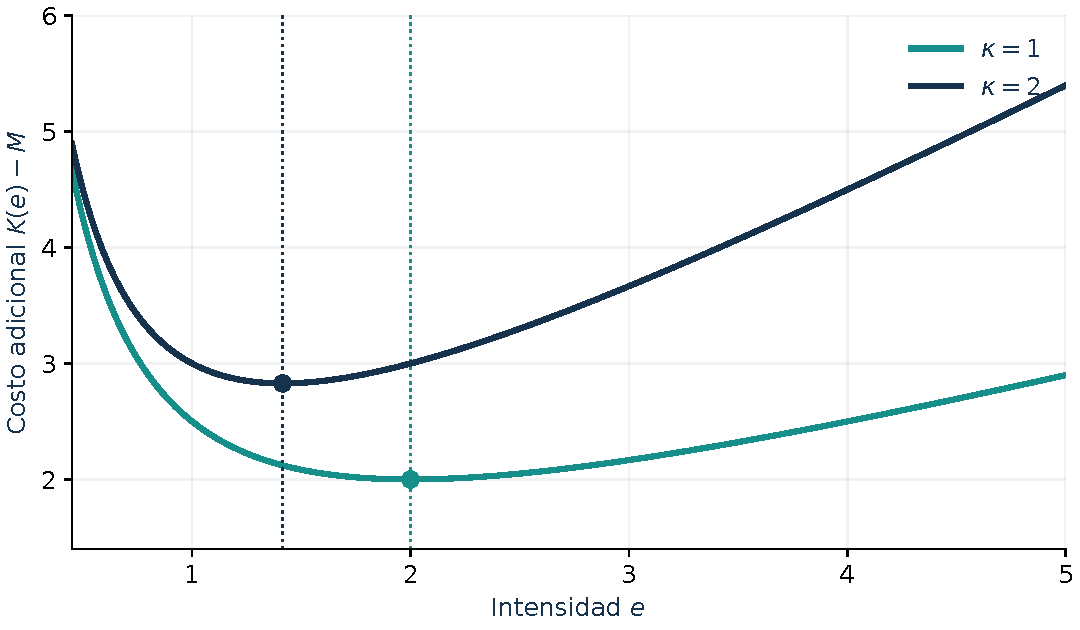
\includegraphics[width=\linewidth]{figures/cost_intensity.pdf}
\end{columns}
\nota{La FOC y la segunda derivada localizan un mínimo. La identidad siguiente prueba globalidad y unicidad. Gráfico con $M=10$, $F=2$.}
\end{frame}

\begin{frame}{Prueba: el mínimo es global y único}
Sea $q=\sqrt{2F/\kappa}>0$. Por definición, $F=\kappa q^2/2$.
\[
\begin{aligned}
K(e;\kappa)-K(q;\kappa)
&=\frac Fe+\frac{\kappa e}{2}
-\left(\frac Fq+\frac{\kappa q}{2}\right)\\[.3em]
&=\frac{\kappa q^2}{2e}+\frac{\kappa e}{2}-\kappa q\\[.3em]
&=\frac{\kappa}{2e}(q^2+e^2-2eq)
=\boxed{\frac{\kappa}{2e}(e-q)^2}.
\end{aligned}
\]
Para todo $e>0$, la diferencia es no negativa; es cero únicamente si $e=q$.
\begin{block}{Conclusión}
$q$ existe, alcanza el mínimo y es el único minimizador global en $e>0$.
\end{block}
\end{frame}

\begin{frame}{Proposición 1: intensidad, duración y costo}
Con A1--A4, $M\ge0$, $F>0$ y $\kappa(p,C)>0$, el único mínimo global satisface
\[
\boxed{e^*=\sqrt{\frac{2F}{\kappa}},\quad
T^*=\sqrt{\frac{\kappa}{2F}},\quad
K^*=M+\sqrt{2F\kappa}.}
\]
Las derivadas respecto de la fricción son
\[
e^*_{\kappa}=-\frac{\sqrt{2F}}{2\kappa^{3/2}}<0,\quad
T^*_{\kappa}=\frac{1}{2\sqrt{2F\kappa}}>0,\quad
K^*_{\kappa}=\sqrt{\frac{F}{2\kappa}}>0.
\]
\begin{center}
\begin{tabular}{lccc}\toprule
Cambio supuesto & $e^*$ & $T^*$ & $K^*$ \\\midrule
$p\uparrow$, si $\kappa_p>0$ & $\downarrow$ & $\uparrow$ & $\uparrow$ \\
$C\uparrow$, si $\kappa_C<0$ & $\uparrow$ & $\downarrow$ & $\downarrow$ \\\bottomrule
\end{tabular}
\end{center}
\end{frame}

\begin{frame}{Prueba de los signos distritales}
\textbf{Regla de la cadena.} Para $x\in\{p,C\}$, con $M$ y $F$ constantes:
\[
\frac{\partial e^*}{\partial x}=e^*_{\kappa}\kappa_x,\qquad
\frac{\partial T^*}{\partial x}=T^*_{\kappa}\kappa_x,\qquad
\frac{\partial K^*}{\partial x}=K^*_{\kappa}\kappa_x.
\]
\begin{columns}[T]
\column{.47\linewidth}
\begin{block}{Si $\kappa_p>0$}
$e_p^*<0$, $T_p^*>0$, $K_p^*>0$.
\end{block}
\column{.47\linewidth}
\begin{block}{Si $\kappa_C<0$}
$e_C^*>0$, $T_C^*<0$, $K_C^*<0$.
\end{block}
\end{columns}
\nota{Ejemplo: $e_p^*=-\sqrt{2F}\,\kappa_p/(2\kappa^{3/2})<0$. Los signos dependen de A4 y no identifican causalidad empírica.}
\end{frame}

\begin{frame}{Simulación de la Proposición 1}
\begin{columns}[T]
\column{.62\linewidth}
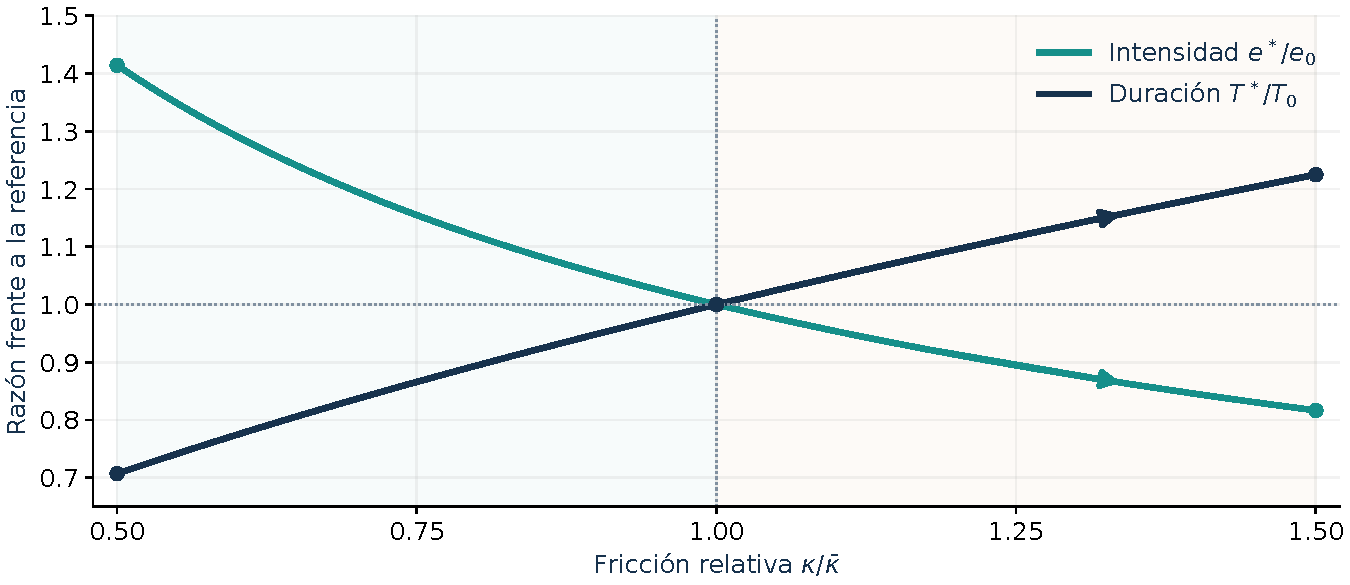
\includegraphics[width=\linewidth]{figures/speed_duration.pdf}
\column{.34\linewidth}
\textbf{Comprueba en el rango mostrado}\par
$e^*/e_0=(\kappa^A/\bar\kappa)^{-1/2}$ cae y
$T^*/T_0=(\kappa^A/\bar\kappa)^{1/2}$ sube.
\medskip

\textbf{No establece}\par
$\kappa_p>0$, causalidad ni magnitudes para el Perú.
\end{columns}
\nota{Ejercicio ilustrativo: $\kappa^A/\bar\kappa\in[0.5,1.5]$. Curvas calculadas con la solución analítica.}
\end{frame}

\begin{frame}{Proposición 2: condición exacta de sobrecosto}
Con A1--A5, $M\ge0$, $F>0$, $\kappa^A,\kappa^V>0$ y el mismo proyecto:
\[
R=\log\!\left(\frac{K^A}{K^V}\right)
=\log\!\left(\frac{M+\sqrt{2F\kappa^A}}{M+\sqrt{2F\kappa^V}}\right).
\]
\[
\boxed{R>0\iff\kappa^A>\kappa^V,\quad
R=0\iff\kappa^A=\kappa^V,\quad
R<0\iff\kappa^A<\kappa^V.}
\]
\begin{block}{Interpretación}
Una obra puede ser lenta y costosa y aun ajustarse al presupuesto si su dificultad se anticipó completamente.
\end{block}
\nota{$\kappa_p^A>0$ sólo implica $R_p>0$ cuando $\kappa^V$ permanece fija.}
\end{frame}

\begin{frame}{Prueba: los tres signos de la variación de costos}
Como $K^V>0$ y $\log$ es estrictamente creciente,
\[R>0\iff \frac{K^A}{K^V}>1\iff K^A>K^V.\]
El costo optimizado crece estrictamente con la fricción:
\[
K^*(\kappa)=M+\sqrt{2F\kappa},\qquad
\frac{\partial K^*}{\partial\kappa}=\sqrt{\frac{F}{2\kappa}}>0.
\]
Por tanto, $K^A>K^V\iff\kappa^A>\kappa^V$. La misma monotonía preserva igualdad y orden inverso:
\[
R=0\iff\kappa^A=\kappa^V,\qquad
R<0\iff\kappa^A<\kappa^V.
\]
\nota{El sobrecosto depende de una brecha respecto de lo anticipado.}
\end{frame}

\begin{frame}{Extensión: anticipación parcial}
\[
\kappa^V(\lambda)=\lambda\kappa^A+(1-\lambda)\bar\kappa,
\qquad\lambda\in[0,1],\quad\bar\kappa>0.
\]
\begin{itemize}
\item $\lambda=0$: el presupuesto usa una fricción genérica $\bar\kappa$.
\item $0<\lambda<1$: incorpora parcialmente la dificultad local.
\item $\lambda=1$: $\kappa^V=\kappa^A$ y $R=0$.
\end{itemize}
Con $\kappa^A$ y $\bar\kappa$ fijas,
\[
R_{\lambda}=
-\frac{\sqrt{F/(2\kappa^V)}}{K^V}
(\kappa^A-\bar\kappa).
\]
\nota{$\lambda$ es exógeno: no representa una decisión óptima ni expectativas racionales.}
\end{frame}

\begin{frame}{Qué implica una mejor anticipación}
\begin{center}
\begin{tabular}{lcc}\toprule
Escenario & Signo de $R$ si $\lambda<1$ & $R_{\lambda}$ \\\midrule
$\kappa^A>\bar\kappa$ & Positivo & Negativo \\
$\kappa^A=\bar\kappa$ & Cero & Cero \\
$\kappa^A<\bar\kappa$ & Negativo & Positivo \\\bottomrule
\end{tabular}
\end{center}
\begin{block}{Resultado}
Cuando $\lambda$ se acerca a 1, $R$ converge a cero desde arriba o desde abajo. La intensidad realizada $e^A$ no cambia porque $\kappa^A$ se mantiene fija.
\end{block}
\nota{Se distingue el costo de ejecutar de la precisión del presupuesto.}
\end{frame}

\begin{frame}{Simulación de la anticipación}
\begin{columns}[T]
\column{.62\linewidth}
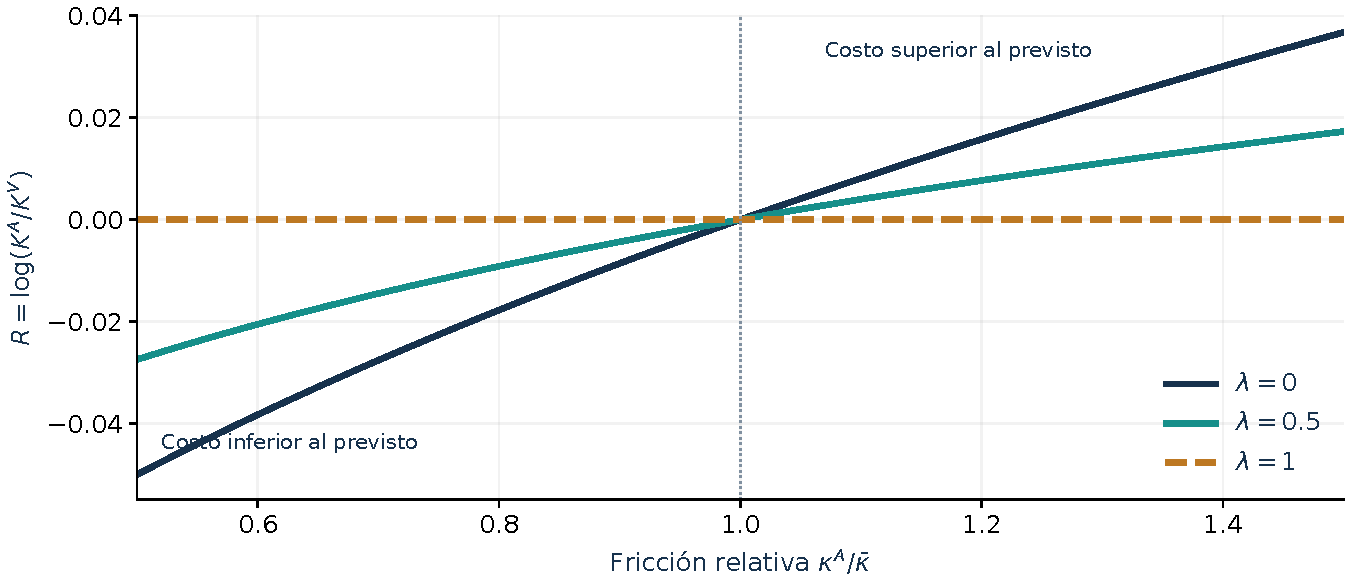
\includegraphics[width=\linewidth]{figures/overrun.pdf}
\column{.34\linewidth}
\textbf{Comprueba}\par
El signo de $R$ a ambos lados de $\kappa^A=\bar\kappa$ y su convergencia a cero cuando $\lambda=1$.
\medskip

\textbf{No identifica}\par
Por qué falla el presupuesto ni el valor empírico de $\lambda$.
\end{columns}
\nota{Escenario ilustrativo: $M=10$, $F=2$, $\bar\kappa=1$; $R$ está en unidades logarítmicas.}
\end{frame}

\begin{frame}{Verificación simbólica y numérica}
\begin{columns}[T]
\column{.47\linewidth}
\textbf{SymPy comprueba}\par
\begin{itemize}
\item FOC en $e^*$ y segunda derivada;
\item identidad $K(e)-K(e^*)=\frac{\kappa}{2e}(e-e^*)^2$;
\item derivadas de $e^*,T^*,K^*$ y $R_{\lambda}$.
\end{itemize}
\column{.47\linewidth}
\textbf{NumPy comprueba en 3000 casos}\par
\begin{itemize}
\item mínimo y comparativas con parámetros positivos;
\item casos $R<0$, $R=0$ y $R>0$;
\item tendencia con $\lambda$ y genera las figuras.
\end{itemize}
\end{columns}
\begin{block}{Alcance}
La prueba algebraica establece las proposiciones. El código detecta errores de derivación o implementación; no estima parámetros peruanos.
\end{block}
\nota{Punto de entrada: \texttt{python code/verify.py}.}
\end{frame}

\begin{frame}{Verificación crítica de una respuesta de IA}
\textbf{Respuesta inicial.} La IA obtuvo $q=\sqrt{2F/\kappa}$ con la FOC. Era necesario verificar que el candidato resolviera el problema global.
\medskip

\textbf{Comprobación manual.} De $F=\kappa q^2/2$ y $K(q)=M+\kappa q$:
\[
\begin{aligned}
K(e)-K(q)
&=\frac{\kappa q^2}{2e}+\frac{\kappa e}{2}-\kappa q\\
&=\frac{\kappa}{2e}(q^2+e^2-2eq)
=\frac{\kappa}{2e}(e-q)^2.
\end{aligned}
\]
\begin{block}{Veredicto}
La fórmula del candidato es correcta. La diferencia de costos demuestra existencia, globalidad y unicidad para $e>0$.
\end{block}
\end{frame}

\begin{frame}{Puente hacia las medidas de la tesis}
\begin{tabular}{p{.24\linewidth}p{.66\linewidth}}
\toprule
Objeto teórico & Medida propuesta en registros administrativos \\\midrule
$e^A=1/T^A$ & Avance financiero dividido entre años desde el primer devengado. \\
$R=\log(K^A/K^V)$ & Logaritmo del costo actualizado sobre el monto viable. \\\bottomrule
\end{tabular}
\medskip
\begin{itemize}
\item La equivalencia de velocidad exige gasto proporcional al avance físico y fechas físicas y financieras alineadas.
\item El costo actualizado puede incluir cambios de alcance y no ser el costo final.
\item Los proyectos en ejecución requieren tratar la censura de duración.
\end{itemize}
\nota{El modelo fija alcance, usa intensidad constante y no incluye una restricción presupuestaria explícita.}
\end{frame}

\begin{frame}{Estado de la prueba y límites abiertos}
\textbf{Demostrado en esta versión}
\begin{itemize}
\item Proposición 1: mínimo global único y signos condicionales.
\item Proposición 2: condición exacta para $R$ positivo, nulo o negativo.
\item Extensión: signo de $R_{\lambda}$ y convergencia a cero.
\end{itemize}
\medskip
\textbf{Para la versión escrita y la discusión empírica}
\begin{itemize}
\item Examinar $\kappa_p>0$ y una medida independiente de $\kappa$.
\item Distinguir progreso físico, financiero y cambios de alcance.
\item Estudiar la decisión de ejecutar, una cota presupuestaria y el valor de terminar antes.
\end{itemize}
\nota{Las pruebas matemáticas dependen de A1--A5; la correspondencia con registros administrativos requiere más trabajo.}
\end{frame}

\begin{frame}{Conclusión y preguntas para la discusión}
\begin{block}{Conclusión}
Más fricción reduce intensidad y eleva duración y costo. Hay sobrecosto si la fricción realizada supera la utilizada en la previsión.
\end{block}
\textbf{Crítica que quisiera recibir de la clase}
\begin{enumerate}\setlength{\itemsep}{.5em}
\item ¿Qué variable aproximaría mejor $\kappa$ sin confundirse con el resultado de ejecución?
\item ¿Conviene relajar primero el alcance fijo o incorporar una restricción presupuestaria?
\item ¿Cómo representar la decisión de ejecutar sin perder la distinción entre fricción y previsión?
\end{enumerate}
\end{frame}

\begin{frame}{Referencias consultadas (1/2)}
\small
\begin{itemize}\setlength{\itemsep}{.55em}
\item Bolo Añorga, C. A. y Roque Tinta, I. M. (2026). \emph{Pobreza y desempeño en la inversión pública en el Perú}. Plan de tesis, 27/09.
\item Loayza, N. V., Rigolini, J. y Calvo-González, O. (2014). More than you can handle: Decentralization and spending ability of Peruvian municipalities. \emph{Economics \& Politics}, 26(1), 56--78.
\item Presbitero, A. F. (2016). Too much and too fast? Public investment scaling-up and absorptive capacity. \emph{Journal of Development Economics}, 120, 17--31.
\item Gurara, D., Kpodar, K., Presbitero, A. F. y Tessema, D. (2020). \emph{On the Capacity to Absorb Public Investment: How Much is Too Much?} FMI WP/20/48.
\end{itemize}
\end{frame}

\begin{frame}{Referencias consultadas (2/2)}
\small
\begin{itemize}\setlength{\itemsep}{.45em}
\item Gambina, D. y Mazzola, F. (2025). The Determinants of the Implementation Speed of Cohesion Projects in Europe: A Regional and Project-level Analysis. \emph{Open Economies Review}.
\item Espinoza, R. y Presbitero, A. F. (2022). Delays in public investment projects. \emph{International Economics}, 172, 297--310.
\item Mohammadi Atashgah, K. et al. (2022). Developing a model for time-cost trade-off optimization problem considering overdraft issue in uncertain environments. \emph{Journal of Industrial and Systems Engineering}, 14(3), 259--279.
\item Flyvbjerg, B., Holm, M. K. S. y Buhl, S. L. (2002). Underestimating costs in public works projects: Error or lie? \emph{Journal of the American Planning Association}, 68(3), 279--295.
\end{itemize}
\end{frame}
\end{document}
